%%%% for public version, toggle \draftfalse in setup2modes.tex
%    (that removes all comments, the blog)

% reducesymm/cgang/2modes.tex    this is master file:    pdflatex 2modes
%     then:    pdflatex def2modes; bibtex def2modes; pdflatex def2modes; pdflatex def2modes

% until 2012-08-20 this was in svn repo siminos/cgang/2modes.tex

\documentclass[aip,cha,
reprint,
secnumarabic,
nofootinbib, tightenlines,
nobibnotes, showkeys, showpacs,
groupedaddress,
%preprint,%
%author-year,%
%author-numerical,%
]{revtex4-1}

\newcommand{\version}{atlas ver. 1.0, Oct  6 2013}
% Predrag                   ver. 0.3, Aug  1 2012
% Predrag                   ver. 0.2, Apr 30 2012}
% Predrag from atlas12      ver. 0.1, Apr 25 2012}

        \input setup2modes
        \input ../inputs/def
        \input def2modes

\begin{document}

\title[Low-dimensional cartography]
{Cartography of a 4-dimensional flow: How to slice and dice it}

\author{Daniel Borrero-Echeverry}
\email{borrero@gatech.edu.}
\author{Burak Budanur}
% \author{Keith M. Carroll} %no response by 2013-08-28
\author{Predrag Cvitanovi\'{c}}
\author{Bryce Robbins} %no response by 2012-07-26, readded 2013-08-28
\author{Evangelos Siminos}
% \author{Lei Zhang} %no response by 2012-07-26, removed
\affiliation{
 School of Physics and Center for Nonlinear Dynamics,
 Georgia Inst. of Technology,
 Atlanta, GA  30332, USA
}
    \ifdraft
\date{\today}
    \else
\date{1 September 2013}
%\affiliation{
% School of Physics and School of Mathematics,
% Georgia Inst. of Technology,
% Atlanta, GA  30332, USA
% \\\\
% Georgia Tech PHYS 7224 spring 2012 course project
% \\
% \emph{Advisers:
% Predrag Cvitanovi\'{c},
% Daniel Borrero-Echeverry
% and
% Evangelos Siminos}
%}
   \fi


    \begin{abstract}
[...]
Such a representation gives rise to an SO(2)-equivariant dynamical system,
trajectories of which are critically effected by the symmetry related structures
such as \reqva\ and \rpo s; thus, the symmetry reduction holds a crucial role
in understanding the dynamics. Method of slices is a technique for reducing
continuous symmetries where one fixes a particular solution as a template in
the \statesp\ and maps nearby solutions onto the hyperplane that is perpendicular
to the group tangent computed at the template point, by acting on them with
the group action. We demonstrate the method of slices by applying it to
radically simple SO(2)-equivariant models where only two Fourier modes are present.
We describe a general two-mode system of order 3, and discuss its representations
in the SO(2)-equivariant state space, in the polar coordinates, and
in an invariant polynomial basis, which enables us to determine all \reqva\ 
of the system. We then focus on two examples with topologically
different chaotic dynamics corresponding to two the different choices of
parameters and apply the method of slices on these systems. We show
that one can determine the symbolic dynamics of
all \rpo s of the system by constructing Poincar\'e
return maps on the slice hyperplane. We can visualise each step of the study
without projecting it onto a sub-manifold since the slice hyperplane, for
this four-dimensional case, is three dimensional.
    \end{abstract}

\pacs{02.20.-a, 05.45.-a, 05.45.Jn, 47.27.ed, 47.52.+j, 83.60.Wc}
\keywords{
symmetry reduction,
equivariant dynamics,
relative equilibria,
relative periodic orbits,
slices,
moving frames
}
\maketitle

%\ifdraft\onecolumngrid % 2012-08-06 temporary \onecolumngrid


    \begin{quotation}
Today, it is possible to  [blah blah].
    \end{quotation}

\section{Introduction}
\label{s:intro}

Over the last decade, new insights into the dynamics of  [blah blah]

Our goals here are two-fold:
    \PC{{\bf[2013-10-07]} Burak's and Daniels outline of Das Artikel is
in \reffig{fig:131007outline}.
}
(i)  Illustrate \mslices\ in the lowest\dmn\ setting possible.
(ii) [blah blah].

As a motivation, consider the chaotic dynamics exhibited by the
small-cell \KS\ system studied in \refref{lanCvit07}. Examination of
typical long-time simulations shows that the spatio-temporal chaos arises
from visits to two kinds of unstable patterns, a `central wobble' region
$S_C$, and a symmetric pair of right/left `drifts' $\{S_L,S_R\}$. In
\statesp\ projections orbits stay in one neighborhood for a while, then
hop to another neighborhood, as illustrated in \reffig{f:antlong}. The
strange attractor that they explore is curved and folded in such a way
that a single local linear chart cannot cover the whole attractor,
several charts are needed, as illustrated by \reffig{fig:2ModeAtlas}\,(d).

The \statesp s of \KS\ and fluid-dynamical flows are high\dmn\ and
difficult to visualize, so here we shall illustrate the key ideas by a
much simpler example, the $\SOn{2}$-equivariant  \twoMode\ system.

%%%%%%%%%%%%%%%%%%%%%%%%%%%%%%%%%%%%%%%%%%%%%%%%%%%%%%%%%%%%
\begin{figure} %[tbp] %[h]
    \centering
% 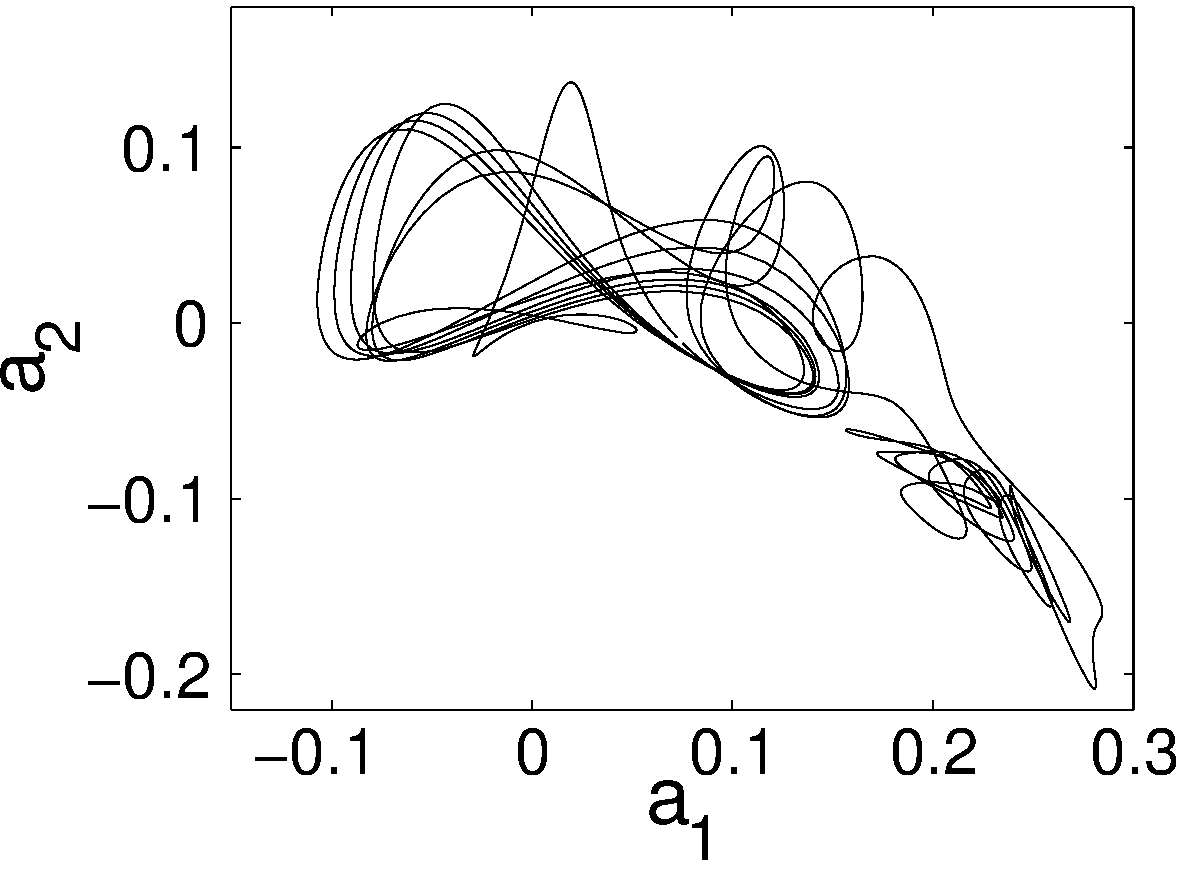
\includegraphics[width=0.40\textwidth]{kslong12}
\caption[]{
A long \KS\ \po\ of period $\period{}=355.34$ that connects
neighborhoods called `$S_C$' and `$S_R$',
(c) $[a_1,a_2]$  projection on the first two spatial Fourier modes
(from \refref{lanCvit07}).
      }
\label{f:antlong}
\end{figure}
%%%%%%%%%%%%%%%%%%%%%%%%%%%%%%%%%%%%%%%%%%%%%%%%%%%%%%%%%%%%%%

%%%%%%%%%%%%%%%%%%%%%%%%%%%%%%%%%%%%%%%%%%%%%%%%%%%%%%%%%%%%%%%%%%%%%
\begin{figure}
%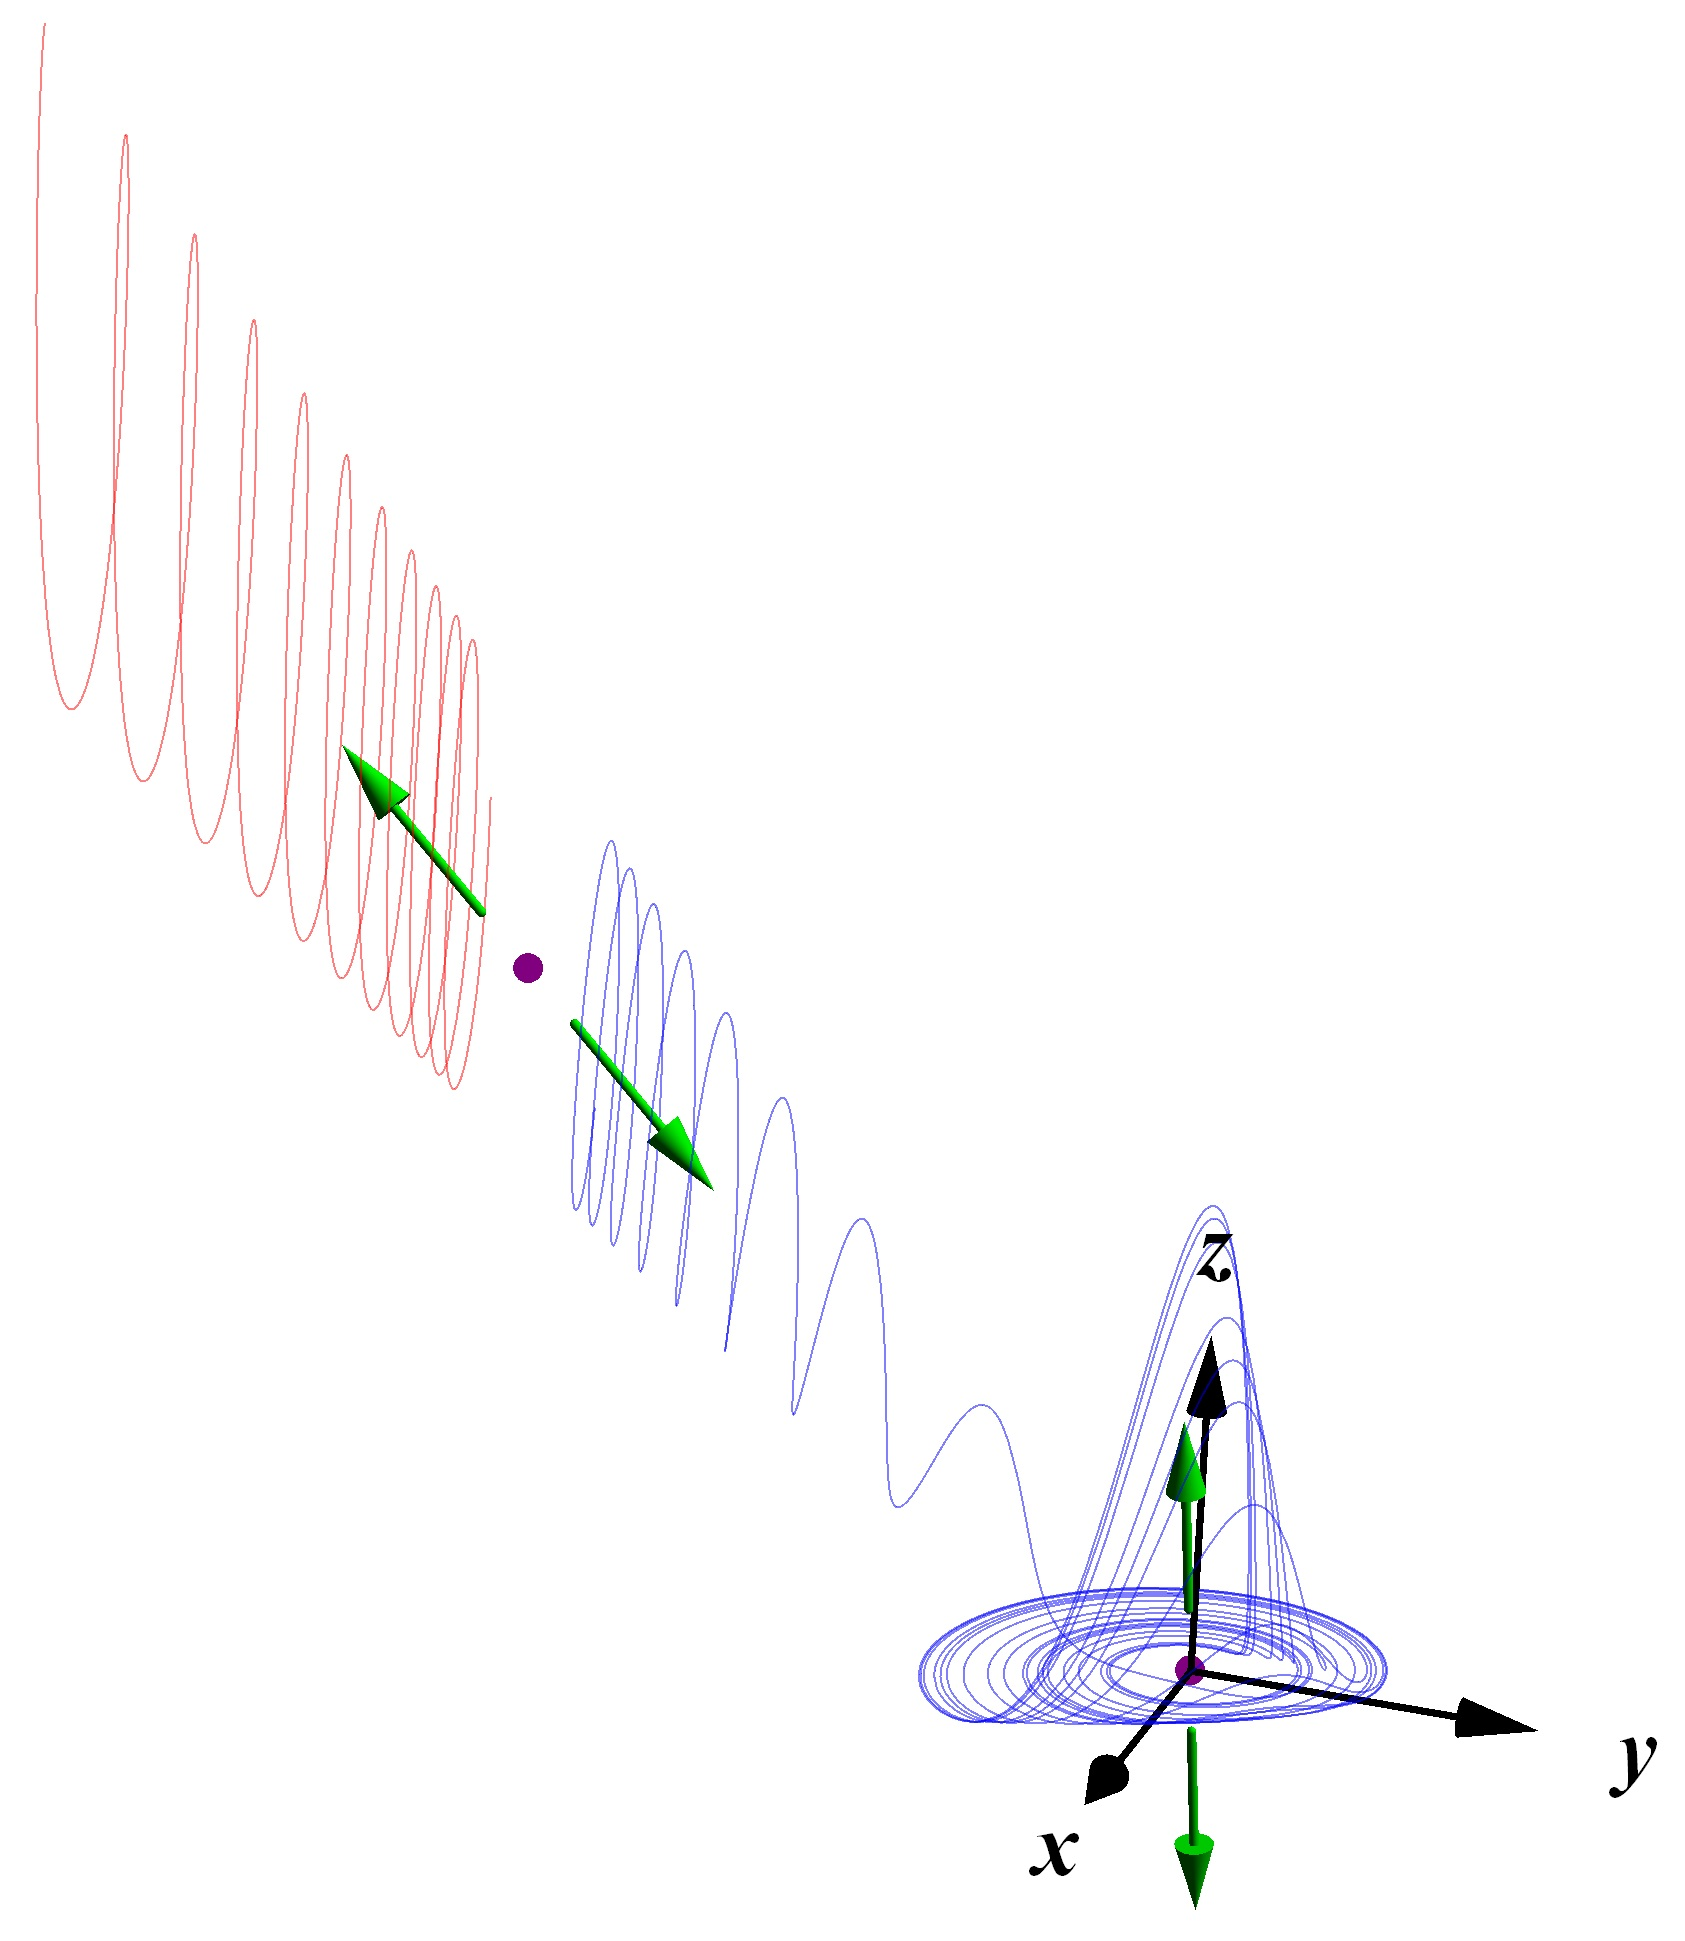
\includegraphics[width=0.28\textwidth]{RoessTrjs2}%{Rossler_Equilibria2}{RoessTrjs}%
 \begin{center}
 \setlength{\unitlength}{0.20\textwidth}
(a)
%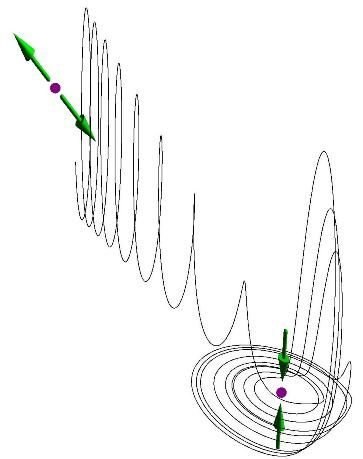
\includegraphics[width=\unitlength,clip=true]{RoessTrajLbld2}
(b)
%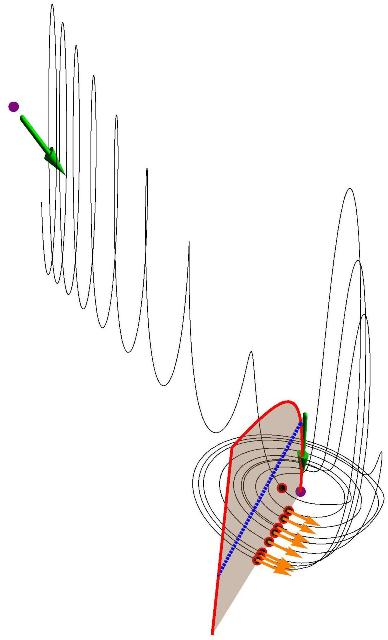
\includegraphics[width=\unitlength,clip=true]{RoessNeareqLbld2}
\\
(c)
%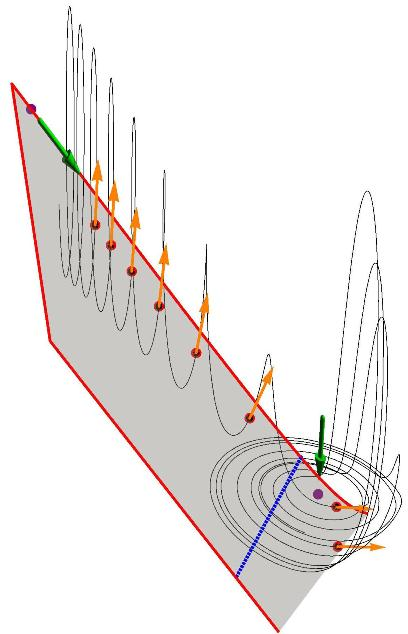
\includegraphics[width=\unitlength,clip=true]{RoessFareqLbld2}
(d)
%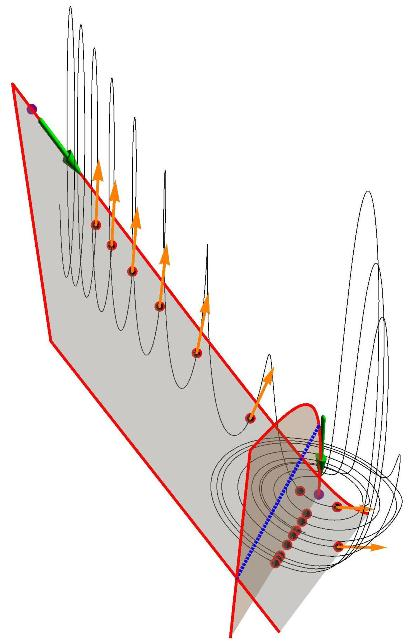
\includegraphics[width=\unitlength,clip=true]{RoessBotheqLbld2}
 \end{center}
    \caption{
2-chart atlas for \twoMode\ flow.
(a)
(b)
(c)
(d)
    }
\label{fig:2modeSects}
\end{figure}
%%%%%%%%%%%%%%%%%%%%%%%%%%%%%%%%%%%%%%%%%%%%%%%%%%%%%%%%%%%%%%%%%%%%%

 [blah blah]

\section{Dynamics and symmetry}
\label{s:symm}

A dynamical system, $\dot{\ssp}=\vel(\ssp)$, is equivariant under a continuous symmetry transformation
$\ssp'= \exp\left( \theta \Lg\right)\ssp$, if it satisfies the equivariance condition \rf{DasBuch}:
\beq
  \groupTan(\vel)  - \Mvar(\ssp) \, \groupTan(\ssp) =0
  \,.
\ee{inftmInv}
Here, $\Mvar(\ssp)_{ij} = {\pde \vel_i}/{\pde\ssp_j} |_x$ is
the \stabmat and $ \groupTan(\ssp) = \Lg \ssp $ is the group tangent evaluated at
the point $\ssp$, whereas $ \groupTan(\vel) = \Lg \vel(\ssp) $ is the group tangent
for the velocity vector evaluated at \ssp . 

For a point $\ssp_\stagn$ in a \reqv\ orbit, the flow and 
group tangent vectors coincide,
\(
\vel = \velRel \, \groupTan(\ssp)
\,.
\)
By symmetry, the \phaseVel\ $\velRel$ is constant. Multiplying the
equivariance condition \refeq{inftmInv} by $\velRel$ we get
\beq
(\velRel \Lg - \Mvar ) \vel =0
\,.
\ee{ReqvMargEig}
In other words, in the co-rotating frame the stability eigenvalue
corresponding to group tangent is marginal, and the velocity
$\vel(\ssp_\stagn)$ is the corresponding right eigenvector.

If a $d$\dmn\ dynamical flow is $\Group$-equivariant under actions of
an $N$ continuous parameters symmetry group $\Group$, its $d$\dmn\ \statesp\ is foliated
by $N$\dmn\ group orbits, and the symmetry-\reducedsp\
$\pS/\Group$ is $(d\!-\!N)$\dmn.
The simplest continuous symmetry groups are the 1-parameter compact rotation
group $\SOn{2}$ and the 1-parameter noncompact translation group
$T(1)$; here we shall focus on the $\SOn{2}$ case.
    \PC{notation for the translation group?}
As at least 3 dimensions are required for a continuous time flow to
exhibit chaos, in this case the \statesp\ of a $\Group$-equivariant flow
has to be at least 4\dmn. Under linear actions of $\SOn{2}$ the \statesp\
decomposes into 2\dmn\ irreducible subspaces (Fourier components) labeled
by integers $m = 0,1,2,\cdots$, which thus form the natural basis in which
to study $\SOn{2}$-equivariant flows. Nonlinear flows, such as the
1 spatial dimension \KS\ PDE for a `flame front velocity' field
$u=u(x,t)$ on a periodic domain $u(x,t) = u(x+L,t)$, given by
\beq
  u_t = F(u) = -{\textstyle\frac{1}{2}}(u^2)_x-u_{xx}-u_{xxxx}
    \,,\qquad   x \in [-L/2,L/2]
    \,,
\ee{BBks1}
can be
expressed in terms of complex Fourier coefficients $a_k(t)$,
\beq
  u(x,t)=\sum_{k=-\infty}^{+\infty} a_k (t) e^{ i q_k x}
\,,\qquad
  q_k = 2\pi k/L
\,,
\ee{BBeq:ksexp1}
as
\beq
\dot{a}_k= \pVeloc_k(a)
     = ( q_k^2 - q_k^4 )\, a_k
    - i \frac{q_k}{2} \sum_{m=-\infty}^{+\infty} a_m a_{k-m}
\,.
\ee{2m:expan}
($t \geq 0$ is the time, $x$ is the spatial coordinate, subscripts $x$
and $t$ denote partial derivatives with respect to $x$ and $t$).
Nonlinear terms mix an infinity of
Fourier components. In practice, they are represented by truncations to
a finite number of Fourier modes; the most radical truncation that
still might capture some qualitative features of a chaotic flow is to keep
only a pair of Fourier modes.


\subsection{\twoMode\ $\SOn{2}$-equivariant flow}
\label{s:twoMode}

Dangelmayr,\rf{Dang86} Armbruster, Guckenheimer and Holmes,\rf{AGHO288}
Jones and Proctor,\rf{JoPro87} and Porter and Knobloch\rf{PoKno05} (see
Golubitsky \etal\rf{golubII}, Sect. XX.1) have investigated bifurcations
in 1:2 resonance ODE normal form models to third order in the amplitudes.
Our starting point is such a model
that we shall refer to as the {\twoMode} system:
\begin{subequations}\label{eq:DangSO2}
\begin{align}
  \dot{z}_1 &= (\mu_1-\ii\, e_1)\,z_1+a_1\,z_1|z_1|^2
  +b_1\,z_1|z_2|^2+c_1\,\overline{z}_1\,z_2
\\
  \dot{z}_2 &= (\mu_2-\ii\, e_2)\,{z_2}+a_2\,z_2|z_1|^2+b_2\,z_2|z_2|^2+c_2\,z_1^2
\,,
\end{align}
\end{subequations}
with $z_1,\,z_2$  complex, and all parameters real valued. The complex
\twoMode\ system \refeq{eq:DangSO2} may be rewritten as a 4-dimensional
first order ODE system,
by substitution $z_1 = x_1 + i\,y_1$, $z_2 = x_2 + i\,y_2$,
\bea
\dot{x}_1 &=& (\mu_1 + a_1 r_1^2 + b_1 r_2^2 + c_1 x_2)x_1 + c_1 y_1 y_2 + e_1 y_1 
\continue
\dot{y}_1 &=& (\mu_1 + a_1 r_1^2 + b_1 r_2^2 - c_1 x_2)y_1 + c_1 x_1 y_2 - e_1 x_1
\continue
\dot{x}_2 &=& (\mu_2 + a_2 r_1^2 + b_2 r_2^2)x_2 + c_2 (x_1^2 - y_1^2) + e_2 y_2
\continue
\dot{y}_2 &=& (\mu_2 + a_2 r_1^2 + b_2 r_2^2)y_2 + 2 c_2 x_1 y_1 - e_2 x_2 
\continue
		  && \mbox{where } r_1^2 = x_1^2 + y_1^2\, , \quad r_2^2 = x_2^2 + y_2^2
\,.
\label{2mode4D}
\eea
As our goal is only to
illustrate and compare continuous symmetry reduction schemes, we shall
study here several simplified versions of model \refeq{eq:DangSO2}, in
the dimensionally lowest possible setting, with the full \statesp\ of
dimension $d=4$, and the $\SOn{2}$-reduced dynamics taking place in 3
dimensions. For these models the
parameters are far from the bifurcation values, and have no
physical interpretation.

It can be checked by inspection that equations \refeq{eq:DangSO2} are
equivariant under the \Un{1}\ transformation
\beq
(z_1,z_2) \rightarrow   (e^{i {\gSpace}}z_1,e^{i 2{\gSpace}} z_2)
\,.
\ee{Dang86(1.1)aa}
In the real representation \refeq{2mode4D}, the $\SOn{2}$ group action
\refeq{Dang86(1.1)aa} is given by $\ssp'= \exp\left( \theta \Lg\right)\ssp$,
where $\transp{\ssp} = \{ x_1, y_1,x_2, y_2\}$, and $\Lg$ is the Lie algebra 
generator
\beq
\Lg  \, =
\left( \begin{array}{cccc}
         0 & 1 & 0 & 0 \\
        -1 & 0 & 0 & 0 \\
         0 & 0 & 0 & 2\\
         0 & 0 & -2 & 0
      \end{array} \right)
\,.
\ee{LGTwoMode}
One can easily check that the real \twoMode\ system \refeq{2mode4D} 
satisfies the equivariance condition \refeq{inftmInv}. 

The parameters $\{e_1,e_2\}$ break the $\On{2}$ symmetry of the
Dangelmayr normal form system\rf{Dang86} to an $\SOn{2}$-equivariant
system. As we show in \refeq{PKinvEqs1} below, only the combination
$(2e_1-e_2)$ matters, so for simplicity we set $e_1=0$. 

From \refeq{eq:DangSO2} we note that the \eqv\ point \((z_1,z_2)=(0,0)\)
is an invariant subspace, and that $z_1=0$, $z_2 \neq 0$ is a 2\dmn\
flow-invariant subspace,
\beq
  \dot{z}_1 = 0
\,,\qquad
  \dot{z}_2 = (\mu_2-\ii\, e_2)\,{z_2}
\,,
\ee{eq:DangSO2spsp}
with a single circular \reqv\ of radius $r_2 = \norm{z_2}$ with
\phaseVel\ $\velRel=e_2$.
    \PC{recheck: is $\velRel=e_2$?}
At the origin $\Mvar$ commutes with $\Lg$, and thus can be block-diagonalized
into two $[2\!\times\!2]$ matrices.
% According to {\bf [2012-04-27 Daniel]},
The $[0,0,0,0]$ \eqv\ eigenvalues are $\lambda_1 = \mu_1$ with multiplicity 2 and
             $\lambda_3 = \mu_2 \pm i e_2$. The eigenvectors for
             $\lambda_1$ are $(1,0,0,0)$ and $(0,1,0,0)$ in the
             $(x_1,x_2,y_1,y_2)$ basis.
             The eigenvectors for
             $\lambda_2$ are $(0,0,1,0)$ and $(0,0,0,1)$



By contrast, for $c_2 \neq 0$, $z_2 =0$ is not a flow-invariant subspace,
as the flow exits the $z_2 =0$ plane,
    \PC{should we check if anything of interest happens for $c_2 = 0$? }
\[
  \dot{z}_1 = (\mu_1-\ii\, e_1)\,z_1+a_1\,z_1|z_1|^2
\,,\qquad
  \dot{z}_2 = c_2\,z_1^2
\,.
\]




\subsection{Invariant polynomial basis}
\label{s:invPol}

% \item[2012-04-28 Predrag]
Consider the \statesp\ of a dynamical system
constructed from two complex Fourier modes
$m=(1,2)$, with the $\SOn{2} \simeq \Un{1}$ group action given by
rotation\rf{Dang86,AGHO288,PoKno05} \refeq{Dang86(1.1)aa}. In this
case it is easy to construct a set of four real
$\SOn{2}$ invariant polynomials
\bea
u &=& {z}_1 \overline{z}_1
    \,,\quad
v = {z}_2 \overline{z}_2
    \continue
w &=& z_1^2 \overline{z}_2 + \overline{z}_1^2 {z}_2
    \,,\quad
q = (z_1^2 \overline{z}_2 - \overline{z}_1^2 {z}_2)/\ii
\,.
\label{Dang86(1.2)PK}
\eea
The polynomials $\{u,v,w,q\}$ are
linearly independent, but related through one syzygy,
%2012-04-29 Double checked, added missing factors of 2 for w and q terms
%2012-04-29 Predrag: thanks!
\beq
w^2+q^2 - 4\,u^2v =0
  \,,
\label{eq:syzPK}
\eeq
which confines the dynamics to a 3-dim\-ens\-ion\-al $\pSRed=\pS/\SOn{2}$
\reducedsp\ manifold, a symmetry-invariant repre\-sent\-ati\-on of the
4-dim\-ens\-ion\-al \SOn{2} equivariant dynamics. By construction $u \geq
0$, $v \geq 0$, but $w$ and $q$ can be of either sign. That is explicit
in in polar coordinates $ {z}_1 = |u|^{1/2} e^{\ii\theta_1}$, $ {z}_2 =
|v|^{1/2} e^{\ii\theta_2}$, where the  $w, q$ invariants take form
\bea
w &=& 2\,\Re(z_1^2 \overline{z}_2) = 2\,u |v|^{1/2} \cos \psi %Double checked DB 04-29-2012
\continue
q &=& 2\,\Im(z_1^2 \overline{z}_2) = 2\,u |v|^{1/2} \sin \psi %Double checked DB 04-29-2012
\,,
\label{Dang86(1.2)polar}
\eea
where $\psi = 2 \theta_1 - \theta_2$.

The dynamical equations for $\{u,v,w,q\}$ follow from the chain rule
\( %beq
 \dot{ u}_i= \sum_j ({\partial u_i}/{\partial \ssp_j}) \, \dot{\ssp}_j
 \,,
\) %ee{HilbChainRl}
upon substitution
$\{{z}_1\,,\overline{z}_1\,, {z}_2\,,\overline{z}_2 \}$ $\to$
$\{u,v,w,q\}$. This yields
\bea
  \dot{u} &=& \overline{z}_1 \dot{z}_1 + {z}_1 \dot{\overline{z}}_1 %Double checked DB 04-29-2012
\,,\qquad
  \dot{v} = \overline{z}_2 \dot{z}_2 + {z}_2 \dot{\overline{z}}_2 %Double checked DB 04-29-2012
\continue
  \dot{w} &=& 2 \,\overline{z}_2 {z}_1 \dot{z}_1 %Double checked DB 04-29-2012
           + 2\,{z}_2 \overline{z}_1 \dot{\overline{z}}_1
           + {z}_1^2 \dot{\overline{z}}_2
           + \overline{z}_1^2 \dot{z}_2
\continue
  \dot{q} &=&  (2\,\overline{z}_2 {z}_1 \dot{z}_1 %Double checked DB 04-29-2012
           - 2\,{z}_2 \overline{z}_1 \dot{\overline{z}}_1
           + {z}_1^2 \dot{\overline{z}}_2
           - \overline{z}_1^2 \dot{z}_2
           )/\ii
\label{PKinvEqs}
\eea
Substituting  \refeq{eq:DangSO2} into \refeq{PKinvEqs} we obtain the set
of 4 $\SOn{2}$-equivariant equations,
%    \PC{2012-04-27 to Lei and all, please recheck! $e_2$ terms differ
%    from Lei. DB 04-29: Double checked using computer algebra. Found a
%    couple of discrepancies. Fixed them in red.}
\bea% Triple checked ES 04-30-2012
  \dot{u} &=& 2\,\mu_1\,u+2\,a_1\,u^2+2\,b_1\,u\,v+c_1\,w %Double checked DB 04-29-2012
\continue
  \dot{v} &=& 2\,\mu_2\,v+2\,a_2\,u\,v+2\,b_2\,v^2+c_2\,w %Double checked DB 04-29-2012
\continue
  \dot{w} &=& (2\,\mu_1+\mu_2)\,w+(2a_1+a_2)\,u\,w+(2b_1+b_2)\,v\,w %Double checked DB 04-29-2012 corrected coefficients for uv and u^2 terms
\ceq
             +\, 4c_1\,u\,v + 2c_2\,u^2 +(2e_1 - e_2)\,q
\label{PKinvEqs1}\\
  \dot{q} &=& (2\mu_1+\mu_2)\,q+(2a_1+a_2)\,u\,q
\ceq
             +(2b_1+b_2)\,v\,q
             -(2e_1-e_2)\,w %Double checked DB 04-29-2012
\,.
\nnu
\eea
Note that the $\On{2}$-symmetry breaking parameters
 $\{e_1,e_2\}$ of the
Dangelmayr normal form system\rf{Dang86} appear only in the
relative phase combination $(2e_1-e_2)$.
%[2012-07-31 Evangelos]
Using the syzygy \refeq{eq:syzPK} we can
eliminate $q$ from \refeq{PKinvEqs} to get
    \PC{
    Note that $4u^2v-w^2 = 4u^2v(1-\cos^2\psi)$, so
    no serious singularity is introduced this way. Perhaps
    write equations of $(u,v,\cos \psi)$ as in the
    ChaosBook exercises?
    }
\bea% Triple checked ES 04-30-2012
  \dot{u} &=& 2\,\mu_1\,u+2\,a_1\,u^2+2\,b_1\,u\,v+c_1\,w %Double checked DB 04-29-2012
\continue
  \dot{v} &=& 2\,\mu_2\,v+2\,a_2\,u\,v+2\,b_2\,v^2+c_2\,w %Double checked DB 04-29-2012
\continue
  \dot{w} &=& (2\,\mu_1+\mu_2)\,w+(2a_1+a_2)\,u\,w+(2b_1+b_2)\,v\,w %Double checked DB 04-29-2012 corrected coefficients for uv and u^2 terms
\ceq
             +\, 4c_1\,u\,v + 2c_2\,u^2 +(2e_1 - e_2)(4u^2v-w^2)^{1/2}\,
\label{PKinvEqs1syz}
\eea

The parameters in \refeq{PKinvEqs1},
with $e_2=0$, $n=2$, $m=1$, are related to the parameters in
equation (2.3) of \refref{Dang86} by $\mu_1=\nu\epsilon\alpha$,
$a_1=-\nu\epsilon$, $b_1=-\nu\epsilon\rho$, $c_1=-\nu\mu$, $\mu_2=\epsilon\beta$,
$a_2=-\epsilon\kappa$, $b_2=-\epsilon\epsilon'$, $c_2=\mu\mu'$.

One can now either investigate the dynamics in this invariant basis or
plot the `image'\rf{GL-Gil07b} of solutions computed in the equivariant
basis \refeq{eq:DangSO2} in terms of invariant polynomials
\refeq{Dang86(1.2)PK}.

%\item[2012-04-29 Predrag]
For the 4\dmn\ model at hand we find the invariant polynomials
and the polar coordinates very useful for cross-checking the
full \statesp\ $\transp{\ssp} = \{ x_1, x_2,y_1, y_2\}$ calculations.
But even
for the simplest conceivable $\SOn{2}$ 4-dimensional flow their
construction requires a bit of algebra, and we do not know
how to carry out such constructions for very high\dmn\ flows,
such as the \KS\ flow \refeq{BBks1}, and the Navier-Stokes flow.


\subsection{\Eqva\ of the symmetry-reduced dynamics}
\label{s:eqva}

The first step in elucidating the geometry of attracting
sets is a determination of their \eqva. For the flows
with velocity fields of multinomial form, the \eqv\
condition $\dot{\sspRed}=0$ reduces to finding roots of
multinomials. We shall now show that the symmetry-reduced
{\twoMode} system
\refeq{PKinvEqs1} has 8 \eqva, real or complex pairs.
%[2012-04-28 Predrag]
How to solve for \eqva\ of \refeq{PKinvEqs}? Define
\beq
A_1= \mu_1+a_1\,u+b_1\,v
    \,,\qquad
A_2 = \mu_2+a_2\,u+b_2\,v
\ee{PKinvEqs2a}
then rewrite \refeq{PKinvEqs} as
%     \newpage
\bea
  0  &=&  2\,A_1\,u +c_1\,w
    \,,\qquad
  0  =  2\,A_2\,v +c_2\,w
\continue
  0  &=& (2\,A_1+ A_2)\,w
             +2\,\left(c_2\,u+2\,c_1\,v\right)\,u -e_2\,q
\label{PKinvEqs3}\\
  0  &=& (2\,A_1+ A_2)\,q + e_2\,\,w
\nnu
\eea
We already know $[0,0,0,0]$ and $[0,v,0,0]$ roots, so we are looking only
for the $u>0$, $v>0$, $w,q \in \reals$ solutions; there could be problems
from the non-generic roots with either $w=0$ or $q=0$, but not both
simultaneously, syzygy \refeq{eq:syzPK} precludes that. $w$ and/or $q$
can be eliminated by rewriting \refeq{PKinvEqs3} as:
\bea
  w  &=& - \frac{2\,u}{c_1}\,A_1 = - \frac{2\,v}{c_2}\,A_2
\continue
        &\to&\quad 2\,A_1+ A_2 = - \frac{ w}{2\,u\,v}\left(c_2\,u+2\,c_1\,v\right)
\continue
  q  &=& \frac{1}{-2e_1+e_2}
     \left(- {w^2}/{2\,u\,v} + \,2u\right)\left(c_2\,u+2\,c_1\,v\right)
\label{PKinvEqs4}\\
  w  &=& -\frac{1}{-2e_1+e_2} (2\,A_1+ A_2)\,q
     \,,\quad\to\quad
  q = \frac{2(-2e_1+\,e_2)\,u\,v}{c_2\,u+2\,c_1\,v}
  \,,
\nnu
\eea
%\DBedit{DB: Not sure where this factor of 2 comes from in $w =
%-\frac{2}{e_2} (2\,A_1+ A_2)\,q $. From the last equation in
%\refeq{PKinvEqs3}, I get $w = -\frac{1}{e_2} (2\,A_1+ A_2)\,q$.
%Therefore, I get I get  $q = \frac{2 e_2\,u\,v}{c_2\,u+2\,c_1\,v}$}
%2012-04-29 Predrag: thanks!
and thus we obtain \textbf{our main result}, two (bivariate)  polynomials
in two variables $\{u,v\}$ with constant coefficients
\bea
f(u,v) &=&
  c_2\,u\,(\mu_1+a_1\,u+b_1\,v)
     -
  c_1\,v\,(\mu_2+a_2\,u+b_2\,v) = 0 %Double checked DB 04-30-2012
\,,\qquad  deg(f) = 2
\continue
g(u,v) &=&
 \left(w^2 - 4\,u^2 v\right)\left(c_2\,u+2\,c_1\,v\right)^2 %Double checked DB 04-30-2012
 +\,4\,(-2e_1+e_2)^2\,u^2\,v^2 = 0
\,,\qquad  deg(g) = 6
\,,
\label{PKinvEqs5}
\eea
% \DBedit{DB: I get $g(u,v) = \left(w^2 - 4\,u^2
% v\right)\left(c_2\,u+2\,c_1\,v\right)^2 +\,4\,e_2^2\,u^2\,v^2 = 0$}
%2012-04-29 Predrag: thanks!
%2012-04-29 Predrag: should have I used the syzygy \refeq{eq:syzPK},
%$w^2 - 4\,u^2v = -q^2$ DB: If you plug the syzygy in you trivially get zero....
where $w$ is defined by the first equation in
\refeq{PKinvEqs4}.
Lots of coefficients, but we can
absorb some into rescaled quantities
$\tilde{u} = c_2\,u$,
$\tilde{v} = c_1\,v$,
$\tilde{a_1} = a_1/c_2$,
$\tilde{b_1} = b_1/c_1$,
$\tilde{a_2} = a_2/c_2$,
$\tilde{b_2} = b_2/c_1$,
and by using $A_1$ expression for $w$ factored out the pair of $u=0$
roots:
\bea
\tilde{f}(\tilde{u},\tilde{v}) &=&
  \tilde{u}\,A_1 - \tilde{v}\,A_2 = 0 %Double checked DB 04-30-2012
\,,\qquad\qquad\qquad  deg(f) = 2
\continue
\tilde{g}(\tilde{u},\tilde{v}) &=&  %Double checked DB 04-30-2012
 \left(A_1^2
 - c_1\,\tilde{v}\right)
 \left(\tilde{u}+2\,\tilde{v}\right)^2
 +e_2^2\,\tilde{v}^2 = 0
\,,\qquad  deg(g) = 4
\continue
 && \mbox{where }
A_1 = \mu_1+\tilde{a_1}\,\tilde{u}+\tilde{b_1}\,\tilde{v}
\,,\quad
A_2 = \mu_2+\tilde{a_2}\,\tilde{u}+\tilde{b_2}\,\tilde{v}
\,,
\label{PKinvEqs5a}
\eea
so we are down to 8 coefficients. Note that $e_2 \in \reals_{+}$, and if
we agree that  $\mu_1 > -\mu_2 > 0$ we can rescale the first equation so
that in new time units $\tilde{\mu}_1 =1$, $\tilde{\mu}_2 = \mu_2/\mu_1
\in \reals_{-}$, so there are 7 coefficients in all. I see no further
rescaling simplification.

As we already know $[0,0,0,0]$ and $[0,v,0,0]$ roots, one should divide
them out, and that is what we have done. Finding
roots of bivariate polynomials is not easy.


%%%%%%%%%%%%%%%%%%%%%%%%%%%%%%%%%%%%%%%%%%%%%%%%%%%%%%%%%%%%%%%%%%%%%%%%%%%%%%%%%%%%%%%%%%%%%%%%%%
\subsection{To do}
\label{s:ToDo}

\begin{itemize}
  \item[10.11] Visualizations of the 4-dimensional {\twoMode} system
  \item[10.1?] draw a group orbit for the {\twoMode} model
  \item[10.22] {\twoMode} system in polar coordinates (maybe skip)
  \item[10.23] The \reqva\ of the {\twoMode} system
  \item[10.24] Plotting the \reqva\ of
           the {\twoMode} system in invariant coordinates
  \item[10.25] Plotting the \reqva\ of
           the {\twoMode} system in Cartesian coordinates
           \refeq{2mode4D}
  \item[10.2?] construct a 2-chart atlas
           \reffig{fig:2ModeAtlas} for a {\twoMode} system
  \item
        compute analytically the \stabmat\ \Mvar\ in polar coordinates
  \item
        Study eigenvalues, keep playing with parameters. We would like
        -preferably- no \reqv\ to be attracting limit cycle, and several of
        the \reqva\ to be complex-pair unstable, leading to chaos, to be
        visualized and sliced in Cartesian coordinates.
  \item
        If you find a nice chaotic attractors, others can join in
        constructing an atlas for it. We just need one and only one
        example with non-trivial \chartBord s and at least 2 charts.
\end{itemize}

 [blah blah]

\begin{itemize}
  \item $\REQV{}{1} = (r_1,r_2,\psi)=(0.0516508, 1.26311,?)$ and
        $\REQV{}{2} = (0.467095,0.2146,?)$
  \item their plots in the Cartesian coordinates
  \item $\dot{\theta}$ to see how slow/fast are they. $\dot{\theta}$
        might be related to 4th eigenvalue, when you go back
        to Cartesian coordinates
  \item stability eigenvalues, eigenvectors of the \eqv\ $\EQV{0}$ at
        origin, at your parameter values - if it is stable, everything
        just might fall into it and die.
  \item plots of small perturbations of the above \eqv\ and \reqva\ in
        the Cartesian coordinates to see whether the dynamics looks
        chaotic
  \item $\REQV{}{1}$: 2 large positive eigenvalues looks scary - probably
        nothing re-visits this \reqv. A mildly unstable complex pair
        would have been sweeter. You get complex eigenvalue by Hopf-bifurcating off a
        stable orbit, typically.
  \item $\REQV{}{1}$: Does either unstable eigenvalue become a complex
        eigenvalue pair in Cartesian coordinates?
  \item $\REQV{}{2}$: contracting eigenvalues have very small imaginary
        part, so the presumably just rocket toward the \reqv, not much
        spiraling there. At least the unstable eigenvalue seems slow
        compared to all other eigenvalues.
  \item $\REQV{}{1}$: Does the unstable eigenvalue become a complex
        eigenvalue pair in Cartesian coordinates?
\end{itemize}

 [blah blah]



%%%%%%%%%%%%%%%%%%%%%%%%%%%%%%%%%%%%%%%%%%%%%%%%%
% 2011-09-09, 2012-03-30 Predrag: add BeThMovFr to
%            continuous.tex overheads, and ChaosBook
% replace A27movFrame*.* everywhere
\begin{figure}
  	\begin{center}
(a)
(b)
(c)
(d)
    \end{center}
  \caption{
  \twoMode, $d=4 \to 3$~dimensional $\{x_1,x_2,z\}$ projections:
  (a)
  The strange attractor.
  (b)
 (c)
 In contrast
 to the 1\dmn\ \poincBord s of \reffig{fig:2modeSects}, here ...
 (d)
  }
\label{fig:2ModeAtlas}
\end{figure}
%%%%%%%%%%%%%%%%%%%%%%%%%%%%%%%%%%%%%%%%%%%%%%%%%%

 [blah blah]

 [blah blah]

\section{Chart}
\label{s:slice}

 [blah blah]

One can write the equations for the flow in the \reducedsp\
$\dot{\sspRed} = \velRed(\sspRed)$ (for details see, for example,
\refref{DasBuch}) as
\bea
\velRed(\sspRed) &=& \vel(\sspRed)
     \,-\, \dot{\gSpace}(\sspRed) \, \groupTan(\sspRed)
\label{2modesEqMotMFrame}\\
\dot{\gSpace}(\sspRed) &=& \braket{\vel(\sspRed)}{\sliceTan{}}
                       /\braket{\groupTan(\sspRed)}{\sliceTan{}}
\,
\label{2modesreconstrEq}
\eea
which confines the motion to the \slice\ hyperplane. Thus, the dynamical
system $\{\pS,\map^t\}$ with continuous symmetry \Group\ is replaced by
the {\reducedsp} dynamics $\{\pSRed,\mapRed^t\}$: The velocity in the
full \statesp\ $\vel$ is the sum of $\velRed$, the velocity component in
the \slice\ hyperplane, and $\dot{\gSpace}\,\groupTan$, the velocity
component along the group tangent space. The integral of the {\em
reconstruction equation} for $\dot{\gSpace}$ keeps track of the group
shift in the full \statesp.


 [blah blah]

\section{Charting the \slice}
\label{s:chart}

Let us summarize the voyage so far:

 [blah blah]


How the charts are put together is best told as a graphic tale, in the 5
frames of Figs.  [blah blah]



\section{Conclusions}
\label{s:concl}

 [blah blah]

\begin{acknowledgments}
This report addresses the questions asked in the  2012 Chaos course
[blah blah].
We are indebted to
Lei Zhang, Bryce Robbins,
    \PC{Is Bryce a co-author or somebody we acknowledge? The time
    will tell}
and
Sarah Flynn
for many inspiring discussions and cross-checks of the model,
and Edgar Knobloch for [...].
\end{acknowledgments}


\bibliography{../bibtex/siminos}
%   \fi % 2012-08-06 end of temporary \onecolumngrid


\ifdraft
    \onecolumngrid

    \newpage
\input flotsam
    \newpage
    \section{{\twoMode} simulations blog}
    \label{chap:Mathematica}
\input ../blog/Mathematica

    \newpage
    \section{{\twoMode} daily blog}
    \label{chap:2modes}
\input ../blog/2modes
    \newpage
    \section{Burak' s {\twoMode}}
    \label{chap:2modesBB}
\input ../blog/2modesBB % Predrag 2013-0810 Burak, git version only

\addcontentsline{toc}{section}{last blog entry}

%\vfill
%\begin{quote}
%{\color{red} \large
%May 1 2012,  11:30am - 2:20pm term projects due, Predrag's office
%}
%\end{quote}

\fi

\end{document}
